\subsection{Построение решения задачи сопряжения гиперболо параболического уравнения с помощью пакета FEniCS}

Рассмотрим следующую задачу сопряжения гиперболо-параболического уравнения:

\begin{equation}
   \pdtt{u_1} = div(gradu_1) + 20t\sin(\pi xy), \quad x \in \Omega_1,~t > 0  
    \label{eq:solution-def-1}
\end{equation}
\begin{equation}
    \pdt{u_2} = div(k_2 grad u_2, \ov n) + 10(t+1)\sin(\pi xy),\quad x\in \Omega_2,~t > 0
    \label{eq:solution-def-2}
\end{equation}

Уравнения (\ref{eq:solution-def-1}) и (\ref{eq:solution-def-2}) дополним граничными условиями Дирихле:
$$ u = 0, \quad x \in \parom $$

На границе раздела задаются условия сопряжения:
$$(gradu_1, \ov n) = (gradu_2, \ov n), \quad x \in \Gamma  $$
$$ u_1(x,t) = u_2(x, t), \quad x \in \Gamma $$

Начальные условия:
$$ u_1(x, 0) = \sin(\pi x)\sin(\pi y), \quad x \in \Omega_1  $$
$$ u_2(x, 0) = (t+1)\sin(\pi x)\sin(\pi y), \quad x \in \Omega_2  $$

$$ \pdt{u_1}(x, 0) = \sin(\pi x)\sin(\pi y), \quad x \in \Omega_1 $$

За область возьмем:
$$ \Omega = [0,1]\times[0,1]$$


На первом слое решение нам уже известно. На втором слое, мы знаем уравнение для $\Omega_1$, для $\Omega_2$ мы строили основное уравнение. Построим триангуляцию области $\Omega$. 

Для начала разобьем область $\Omega$ на $\Omega_1$ и $\Omega_2$, с границей сопряжения $\Gamma$ в точке $x = 0.5$.~(Рисунок 2)

\begin{figure}[H]
      \centering
      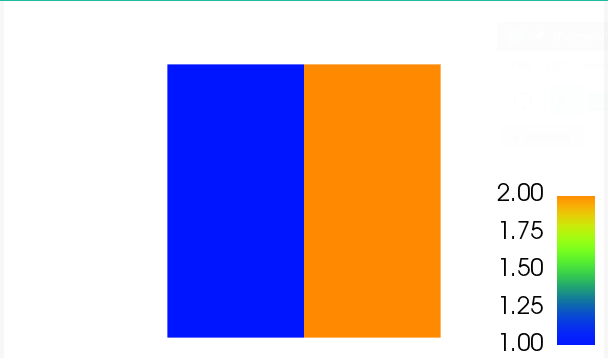
\includegraphics[width=0.8\textwidth]{plots/domains.png}\\
      \centering\caption*{Рисунок 2 -- Рассчетная область $\Omega$ с обозначенными синим цветом $\Omega_1$, оранжевым - $\Omega_2$}
\end{figure}

Проведем триангуляцию области $n=100$ треугольниками и построим решение на первом временном слое, при $t=0$.~(Рисунок 3):
\begin{figure}[H]
      \centering
      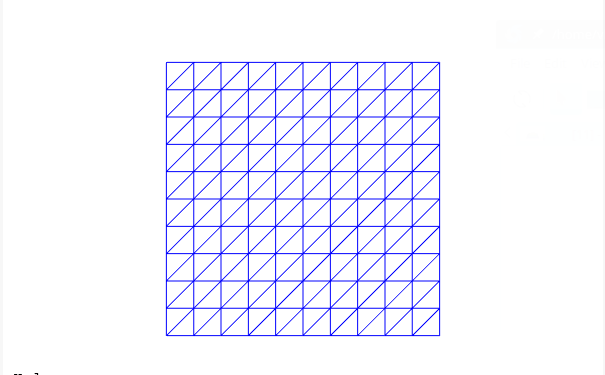
\includegraphics[width=0.8\textwidth]{plots/n10t10_polygons.png}\\
      \centering\caption*{Рисунок 3. -- Триангуляция области $\Omega$ при $n=100$}
\end{figure}

Пример решения на $n=100$ треугольниках и при $t=10$ приведен на рисунке 4:
\begin{figure}[H]
      \centering
      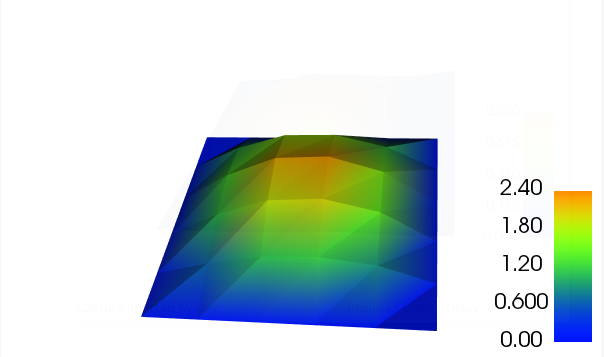
\includegraphics[width=0.8\textwidth]{plots/n10t10.png}\\
      \centering\caption*{Рисунок 4 -- Решение задачи (\ref{eq:solution-def-1})-(\ref{eq:solution-def-2}) при $t=0$}
\end{figure}

Триангуляция $\Omega$ при 400 треугольниках. (Рисунок 5)
\begin{figure}[H]
      \centering
      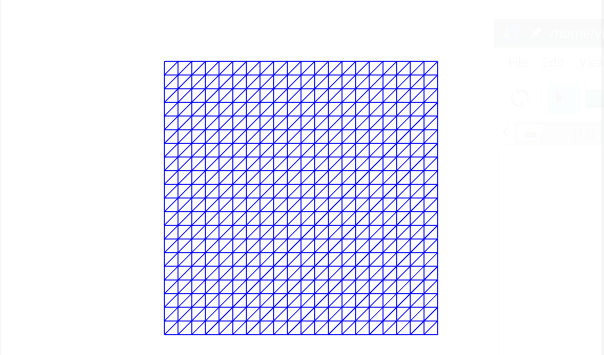
\includegraphics[width=0.8\textwidth]{plots/n20t0_polygons.png}\\
      \centering\caption*{Рисунок 5 -- Триангуляция области $\Omega$ при $n=400$}
\end{figure}

Решение (\ref{eq:solution-def-1})-(\ref{eq:solution-def-2}) начальном временном слое. (Рисунок 6)
\begin{figure}[H]
      \centering
      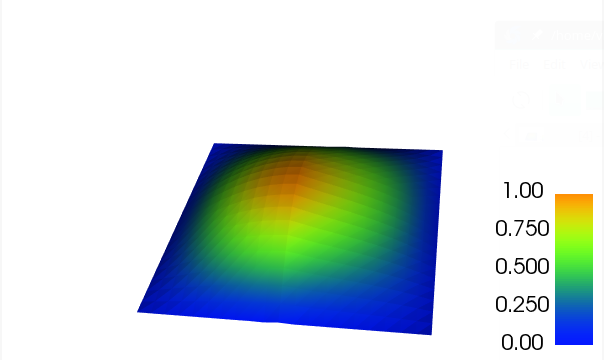
\includegraphics[width=0.8\textwidth]{plots/n20t0.png}\\
      \centering\caption*{Рисунок 6 -- Решение задачи (\ref{eq:solution-def-1})-(\ref{eq:solution-def-2}) при $t=0$, $n=400$}
\end{figure}

Решение задачи (\ref{eq:solution-def-1})-(\ref{eq:solution-def-2}) при 400 треугольниках и $t=10$. (Рисунок 7)
\begin{figure}[H]
      \centering
      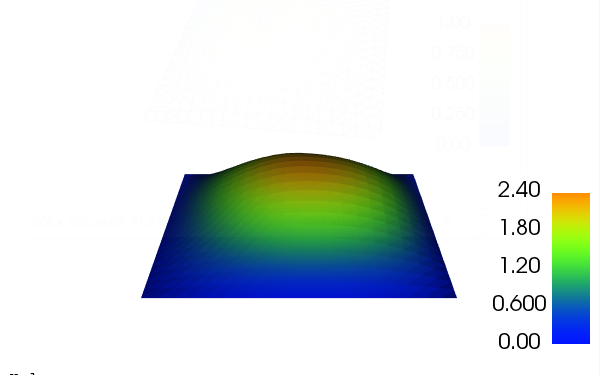
\includegraphics[width=0.8\textwidth]{plots/n20t10.png}\\
      \centering\caption*{Рисунок 7 -- Решение задачи (\ref{eq:solution-def-1})-(\ref{eq:solution-def-2}) при $t=10$, $n=400$}
\end{figure}

Решение на $t=100$, при триангуляции 10000 треугольниками(Рисунок 9). Триангуляция приведедена на рисунке 8:
\begin{figure}[H]
      \centering
      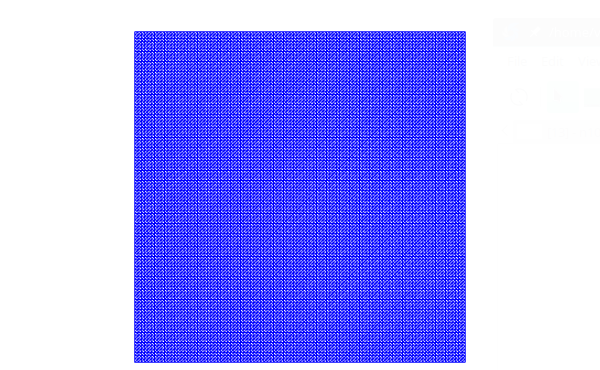
\includegraphics[width=0.8\textwidth]{plots/n100_polygons.png}\\
      \centering\caption*{Рисунок 8 -- Триангуляция области $\Omega$ при $n=10000$}
\end{figure}
\begin{figure}[H]
      \centering
      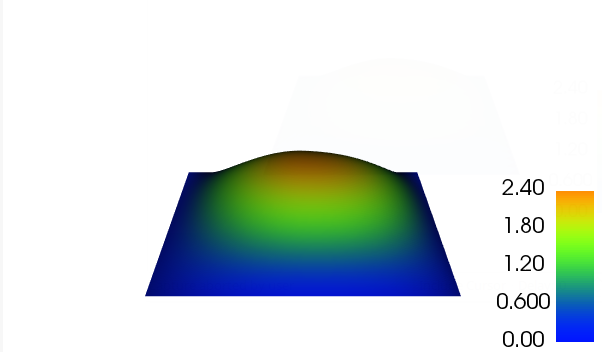
\includegraphics[width=0.8\textwidth]{plots/n100t10.png}\\
  \centering\caption*{Рисунок 9 -- Решение задачи (\ref{eq:solution-def-1})-(\ref{eq:solution-def-2}) при $t=10$, $n=10000$}
\end{figure}

Проведем исследование погрешности по формулам (\ref{eq:kp}) и порядок метода (\ref{eq:mke-level}). Коэффициент $k$ возьмем равным $\frac{1}{2}$,
а константу $M=1$\\
\newpage
\begin{table}
    \begin{center}
        \begin{tabular}{ | l | l | l | p{5cm} |}
            \hline
            n треугольников & $||u||$ \\ \hline
            100 &  1.847176 \\
            400 & 1.89189 \\
            1600 & 1.903268 \\
            \hline
        \end{tabular}
        \caption{Норма найденного решения при различных $n$}
    \end{center}
\end{table}
Итого получили $E_0=0.025$, и порядок метода $p=2$.
\newpage
